\chapter{Metodologia e desenvolvimento}
\label{cap:metodologia}

\section{Ambiente e ferramentas}
Utilizou-se o Compiler Explorer (Godbolt) \cite{godbolt} para compilar o mesmo código em C para duas arquiteturas. Os compiladores foram o \textit{x86-64 gcc 16.1} e o \textit{ARM64 GCC 16.1.0}, da mesma família e versão principal, para que a diferença observada venha da arquitetura e não do compilador. Foram usados os níveis de otimização \texttt{-O0} e \texttt{-O2}. O acesso à ferramenta ocorreu em 4 de novembro de 2026.

\section{Arquiteturas selecionadas}
Foram selecionadas a arquitetura x86-64, classificada como CISC, e a ARM64, classificada como RISC \cite[p.~23--28]{stallings2017}\cite[p.~31--36]{tanenbaum2013}. Em processadores modernos essa distinção é sutil, como discutido no Capítulo~\ref{cap:fundamentacao}.

\section{Código-fonte em C}
O trecho analisado soma os elementos positivos de um vetor. Ele reúne laço de repetição, condição, leitura da memória e acumulação em uma variável.

\lstinputlisting[style=cstyle, caption={Código em C da PoC}, label={lst:c}]{poc/c/soma_positivos.c}

\section{Assembly gerado}
\subsection{x86-64}
\lstinputlisting[style=x86, caption={Assembly x86-64, gcc 16.1, -O0}, label={lst:x86o0}]{poc/asm/x86-64_O0.s}
\lstinputlisting[style=x86, caption={Assembly x86-64, gcc 16.1, -O2}, label={lst:x86o2}]{poc/asm/x86-64_O2.s}

\subsection{ARM64}
\lstinputlisting[style=arm, caption={Assembly ARM64, gcc 16.1.0, -O0}, label={lst:armo0}]{poc/asm/arm64_O0.s}
\lstinputlisting[style=arm, caption={Assembly ARM64, gcc 16.1.0, -O2}, label={lst:armo2}]{poc/asm/arm64_O2.s}

\subsection{Comentários sobre as listagens}
\textbf{x86-64, \texttt{-O0}.} Todas as variáveis ficam na pilha, acessadas por endereços relativos a \texttt{rbp}. O prólogo \texttt{push rbp} e \texttt{mov rbp, rsp} monta o quadro de pilha. O teste do \texttt{for} vira \texttt{cmp} seguido de \texttt{jl .L4}, e o \texttt{if} vira \texttt{test} seguido de \texttt{jle .L3}, que salta sobre a soma quando o elemento não é positivo. A acumulação é feita por \texttt{add DWORD PTR [rbp-4], eax}, uma única instrução que lê e escreve a memória.

\textbf{ARM64, \texttt{-O0}.} O quadro de pilha é reservado por \texttt{sub sp, sp, \#32}. Apenas \texttt{ldr}, \texttt{ldrsw} e \texttt{str} acessam a memória; \texttt{add}, \texttt{lsl} e \texttt{cmp} operam sobre registradores. O endereço de \texttt{v[i]} é calculado por \texttt{lsl} e \texttt{add}. O \texttt{for} vira \texttt{cmp} e \texttt{blt .L4}, e o \texttt{if} vira \texttt{cmp} e \texttt{ble .L3}. A mesma acumulação exige três instruções: \texttt{ldr}, \texttt{add} e \texttt{str}.

\textbf{x86-64, \texttt{-O2}.} As variáveis passam para registradores e a pilha deixa de ser usada. O \texttt{if} não gera salto: \texttt{test eax, eax} e \texttt{cmovs eax, ecx} substituem o valor por zero quando ele é negativo. O laço percorre o vetor por ponteiro, com \texttt{add rdi, 4} e \texttt{cmp rdi, rsi} seguido de \texttt{jne .L4}. O único acesso à memória é \texttt{mov eax, DWORD PTR [rdi]}.

\textbf{ARM64, \texttt{-O2}.} A instrução \texttt{ldr w2, [x3], 4} carrega o elemento e avança o ponteiro em uma só operação (pós-incremento). O \texttt{if} também some como salto: \texttt{bic w2, w2, w2, asr \#31} zera os valores negativos. O laço fecha com \texttt{cmp x3, x1} e \texttt{bne .L4}.

\section{Passo a passo da PoC}
\begin{enumerate}
  \item Abrir o Compiler Explorer e escolher a linguagem C.
  \item Colar o código do Código~\ref{lst:c} no editor.
  \item Selecionar o compilador x86-64 gcc 16.1 e informar a opção \texttt{-O0}.
  \item Adicionar um segundo painel de compilação (\textit{Add new}) com o ARM64 GCC 16.1.0 e a mesma opção \texttt{-O0}.
  \item Copiar o Assembly de cada painel e salvar em arquivo.
  \item Repetir os passos 3 a 5 com a opção \texttt{-O2}.
  \item Registrar a tela de cada configuração (Figuras~\ref{fig:godbolt_o0} e \ref{fig:godbolt_o2}).
\end{enumerate}

\begin{figure}[htb]
  \caption{Compiler Explorer com x86-64 e ARM64, opção -O0}
  \label{fig:godbolt_o0}
  \centering
  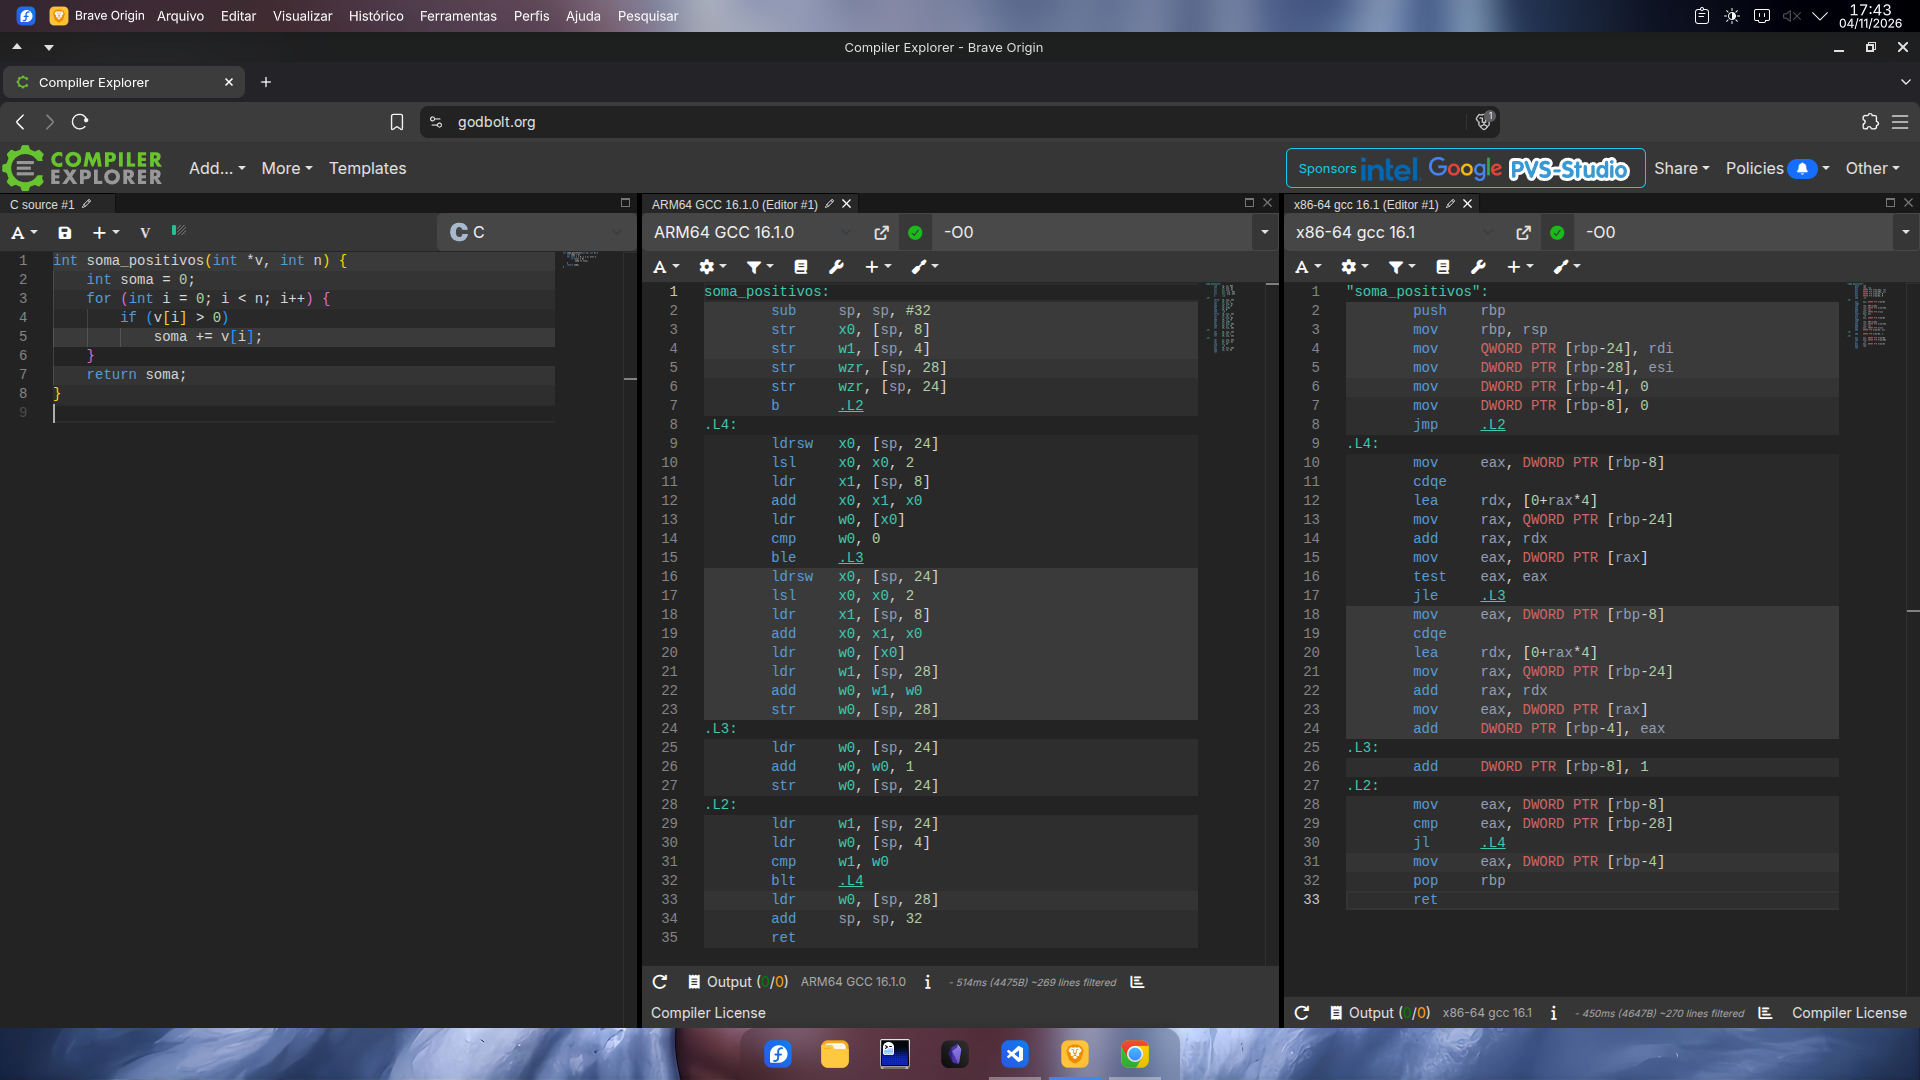
\includegraphics[width=\textwidth]{poc/capturas/godbolt_O0.png}
  \legend{Fonte: elaborado pelos autores no Compiler Explorer.}
\end{figure}

\begin{figure}[htb]
  \caption{Compiler Explorer com x86-64 e ARM64, opção -O2}
  \label{fig:godbolt_o2}
  \centering
  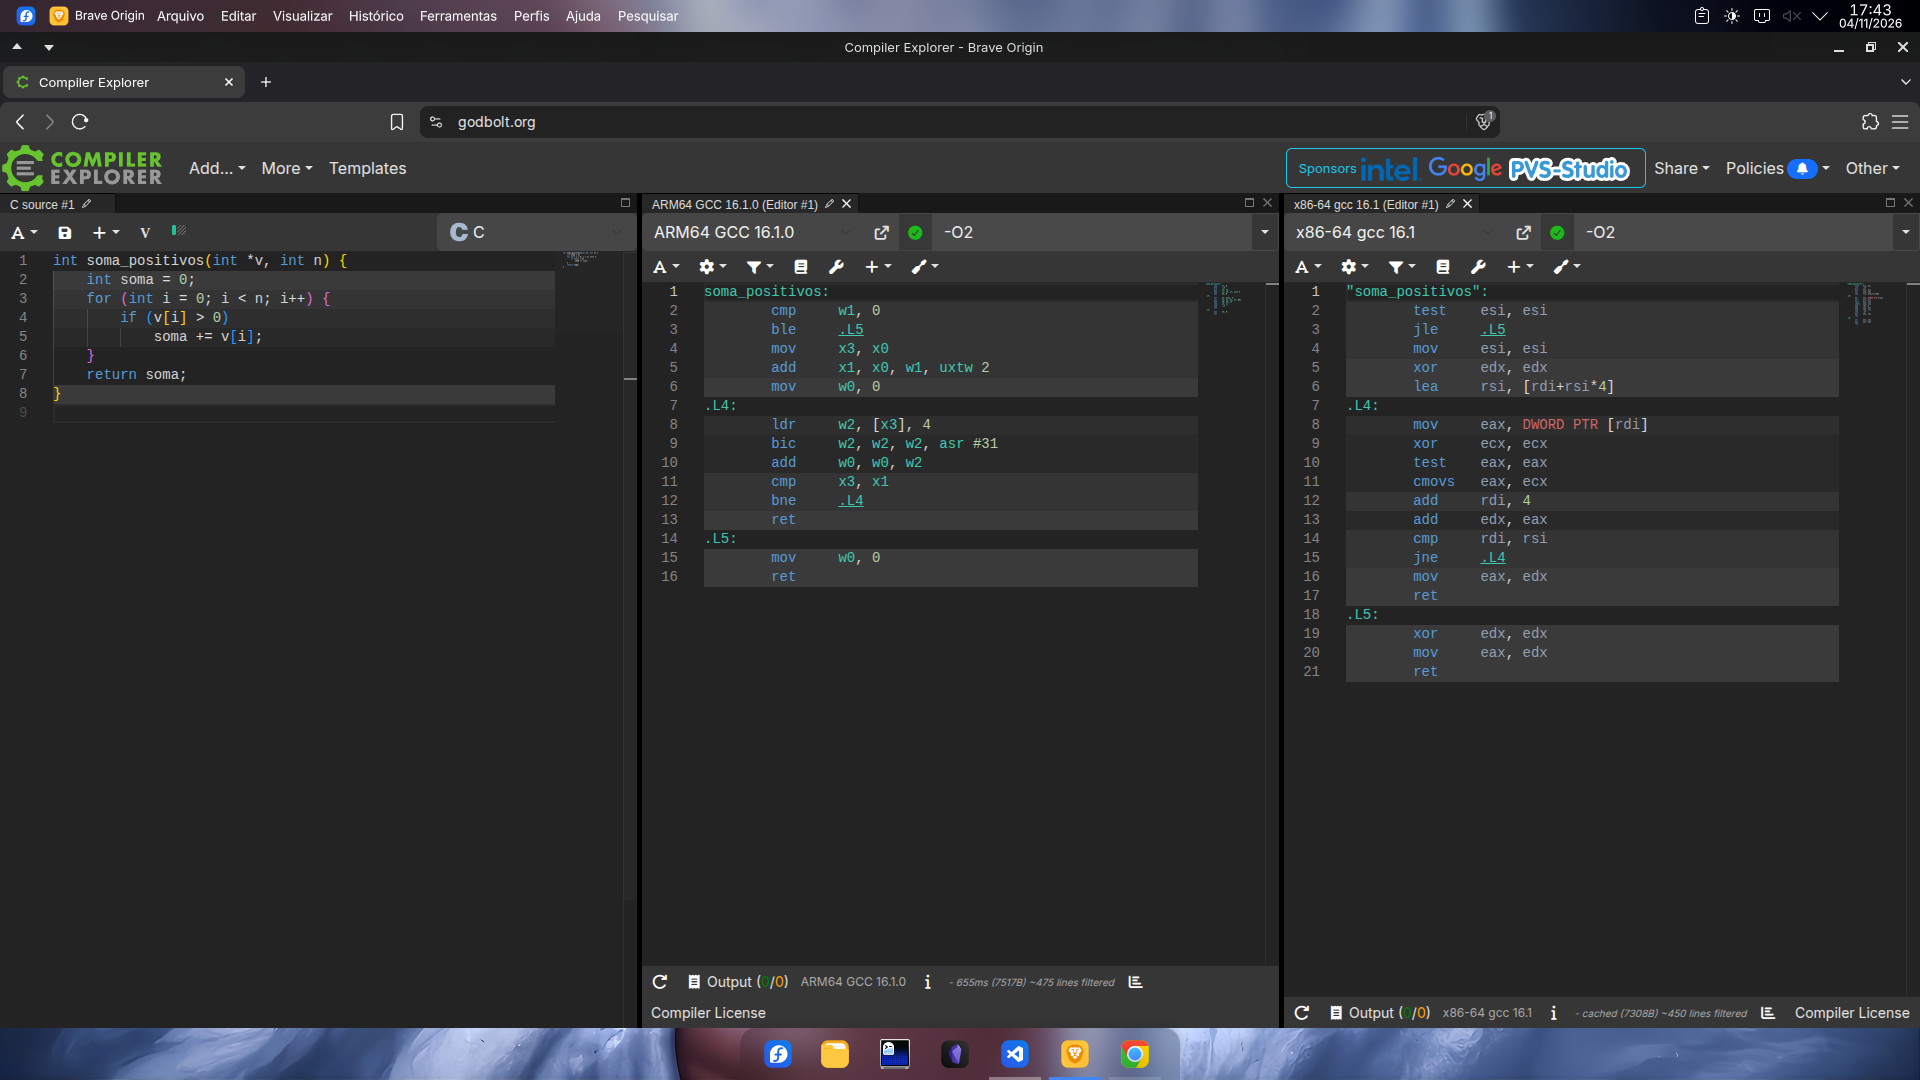
\includegraphics[width=\textwidth]{poc/capturas/godbolt_O2.png}
  \legend{Fonte: elaborado pelos autores no Compiler Explorer.}
\end{figure}

\section{Métricas coletadas}
Foram coletadas métricas estáticas, contadas sobre o texto do Assembly gerado:
\begin{itemize}
  \item \textbf{Instruções:} linhas de instrução, sem contar rótulos e o nome da função. O retorno é contado.
  \item \textbf{Saltos:} instruções de desvio condicional e incondicional. O retorno não é contado.
  \item \textbf{Acessos à memória:} em ARM64, as instruções de carga e armazenamento. Em x86-64, as instruções com operando de memória, exceto \texttt{lea}, que apenas calcula o endereço.
  \item \textbf{Registradores utilizados:} registradores de uso geral distintos, tratando as visões de 32 e 64 bits como um só registrador (por exemplo, \texttt{eax} e \texttt{rax}). Ponteiro de pilha (\texttt{sp}, \texttt{rsp}) e registrador zero (\texttt{wzr}) não são contados; o \texttt{rbp}, usado como base do quadro de pilha, é contado.
  \item \textbf{Bytes de código:} tamanho da função lido na saída binária do Compiler Explorer. Em ARM64, cada instrução ocupa 4 bytes; em x86-64, o tamanho varia. Em \texttt{-O2}, os bytes incluem 3 instruções \texttt{nop} de alinhamento em cada arquitetura, que não entram na contagem de instruções.
\end{itemize}
Os valores estão na Tabela~\ref{tab:comparacao}, no Capítulo~\ref{cap:discussao}.

\section{Limitação do método}
O Godbolt realiza análise estática. Ele mostra as instruções geradas, mas não executa o programa e não mede ciclos reais. Contagem de instruções não equivale a desempenho. Os resultados valem para este trecho de código e para as versões de compilador usadas.